\documentclass{article}
\usepackage[utf8]{inputenc}

\usepackage{tikz}
\usetikzlibrary{automata, positioning, arrows}

\begin{document}
\ \\
\textbf{
Finite automata for the examples of symetric difference and weight of a language.}

\begin{figure}[h!]
	\centering
	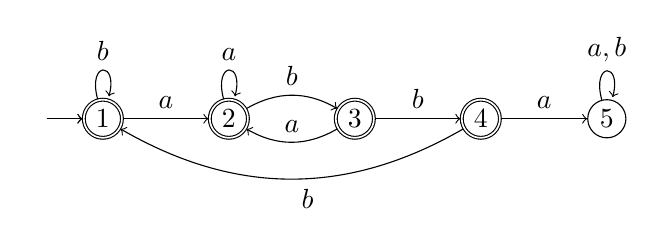
\begin{tikzpicture}[node distance=16mm, every state/.style={minimum size=4mm, inner sep=2pt}]
		\node[state,initial,initial,initial text={},accepting] (1) {$1$};
		\node[state,accepting] (2)  [right of=1]  {$2$};
		\node[state,accepting] (3) [right of=2] {$3$};
		\node[state,accepting] (4)  [right of=3]  {$4$};
		\node[state] (5)  [right of=4]  {$5$};
		
		\path[->] 
		(1) edge [loop above] node {$b$} ()
		(1) edge node [above] {$a$} (2)
		(2) edge [loop above] node {$a$} ()
		(2) edge [bend left] node [above] {$b$} (3)
		(3) edge [bend left] node [above] {$a$} (2)
		(3) edge node [above] {$b$} (4)
		(4) edge [bend left] node [below right] {$b$} (1)
		(4) edge node [above] {$a$} (5)
		(5) edge [loop above] node [above] {$a,b$} ();
	\end{tikzpicture}
\caption{solution}
\label{fig:nfa_no_abba}
\end{figure}


\begin{figure}[h!]
	\centering
	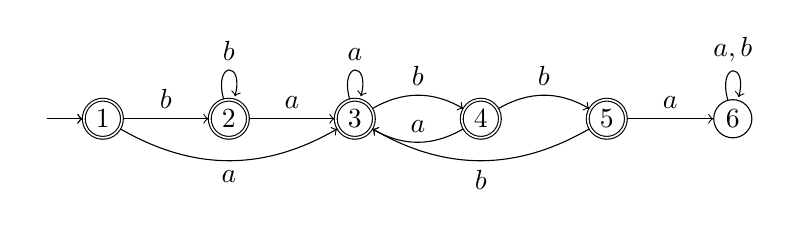
\begin{tikzpicture}[node distance=16mm, every state/.style={minimum size=4mm, inner sep=2pt}]
		\node[state,initial,initial,initial text={},accepting] (1){$1$};
		\node[state,accepting] (2) [right of=1]{$2$};
		\node[state,accepting] (3) [right of=2]{$3$};
		\node[state,accepting] (4) [right of=3]{$4$};
		\node[state,accepting] (5) [right of=4]{$5$};
		\node[state] (6) [right of=5]{$6$};
		
		\path[->] 
		(1) edge node [above] {$b$} (2)
		(2) edge [loop above] node {$b$} ()
		(2) edge node [above] {$a$} (3)
		(3) edge [loop above] node {$a$} ()
		(3) edge [bend left] node [above] {$b$} (4)
		(4) edge [bend left] node [above] {$a$} (3)
		(4) edge [bend left] node [above] {$b$} (5)
		(5) edge [bend left] node [below] {$b$} (3)
		(1) edge [bend right] node [below] {$a$} (3)
		(5) edge node [above] {$a$} (6)
		(6) edge [loop above] node [above] {$a,b$} ();
	;
	\end{tikzpicture}
\caption{automaton1}
\label{fig:error_1}
\end{figure}


\begin{figure}[h!]
	\centering
	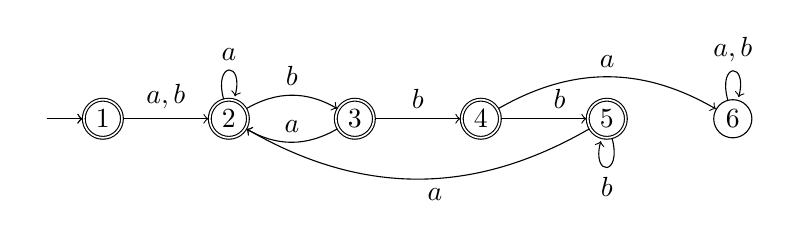
\begin{tikzpicture}[node distance=16mm, every state/.style={minimum size=4mm, inner sep=2pt}]
		\node[state,initial,initial,initial text={},accepting] (1) {$1$};
		\node[state,accepting] (2)  [right of=1]  {$2$};
		\node[state,accepting] (3) [right of=2] {$3$};
		\node[state,accepting] (4)  [right of=3]  {$4$};
		\node[state,accepting] (5)  [right of=4]  {$5$};
		\node[state] (6) [right of=5]{$6$};
		
		\path[->] 
		(1) edge node [above] {$a, b$} (2)
		(2) edge [loop above] node {$a$} ()
		(2) edge [bend left] node [above] {$b$} (3)
		(3) edge [bend left] node [above] {$a$} (2)
		(3) edge node [above] {$b$} (4)
		(4) edge node [above right] {$b$} (5)
		(5) edge [loop below] node [below] {$b$} ()
		(5) edge [bend left] node [below right] {$a$} (2)
		(4) edge [bend left] node [above] {$a$} (6)
		(6) edge [loop above] node [above] {$a,b$} ();
	\end{tikzpicture}
\caption{automaton2}
\label{fig:error_2}
\end{figure}

\begin{figure}[h!]
	\centering
	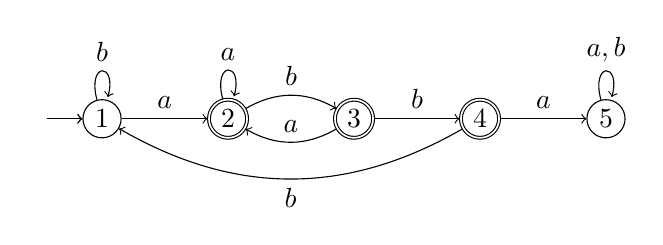
\begin{tikzpicture}[node distance=16mm, every state/.style={minimum size=4mm, inner sep=2pt}]
		\node[state,initial,initial,initial text={}] (1) {$1$};
		\node[state,accepting] (2)  [right of=1]  {$2$};
		\node[state,accepting] (3) [right of=2] {$3$};
		\node[state,accepting] (4)  [right of=3]  {$4$};
		\node[state] (5)  [right of=4]  {$5$};
		
		\path[->] 
		(1) edge [loop above] node {$b$} ()
		(1) edge node [above] {$a$} (2)
		(2) edge [loop above] node {$a$} ()
		(2) edge [bend left] node [above] {$b$} (3)
		(3) edge [bend left] node [above] {$a$} (2)
		(3) edge node [above] {$b$} (4)
		(4) edge [bend left] node [below] {$b$} (1)
		(4) edge node [above] {$a$} (5)
		(5) edge [loop above] node [above] {$a,b$} ();
	\end{tikzpicture}
\caption{automaton3}
\label{fig:error_3}
\end{figure}

\begin{figure}[h!]
	\centering
	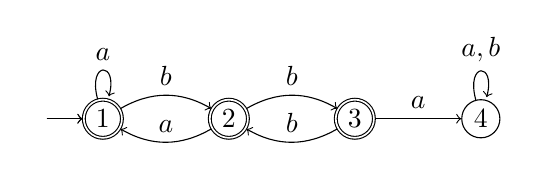
\begin{tikzpicture}[node distance=16mm, every state/.style={minimum size=4mm, inner sep=2pt}]
		\node[state,initial,initial,initial text={},accepting] (1) {$1$};
		\node[state, accepting] (2)  [right of=1]  {$2$};
		\node[state, accepting] (3) [right of=2] {$3$};
		\node[state] (4)  [right of=3]  {$4$};
		
		\path[->] 
		(1) edge [loop above] node {$a$} ()
		(1) edge [bend left] node [above] {$b$} (2)
		(2) edge [bend left] node [above] {$a$} (1)
		(3) edge [bend left] node [above] {$b$} (2)
		(2) edge [bend left] node [above] {$b$} (3)
		(3) edge node [above] {$a$} (4)
		(4) edge [loop above] node [above] {$a,b$} ();
	\end{tikzpicture}
\caption{automaton4}
\label{fig:error_5}
\end{figure}

\begin{figure}[h!]
	\centering
	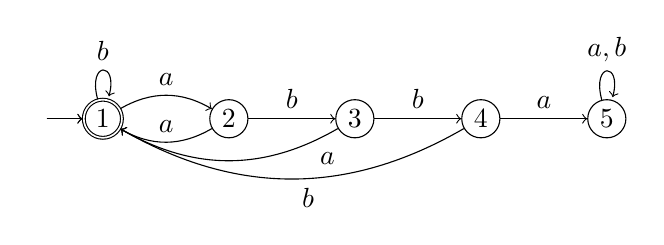
\begin{tikzpicture}[node distance=16mm, every state/.style={minimum size=4mm, inner sep=2pt}]
		\node[state,initial,initial,initial text={},accepting] (1) {$1$};
		\node[state] (2)  [right of=1]  {$2$};
		\node[state] (3) [right of=2] {$3$};
		\node[state] (4)  [right of=3]  {$4$};
		\node[state] (5)  [right of=4]  {$5$};
		
		\path[->] 
		(1) edge [loop above] node {$b$} ()
		(1) edge [bend left] node [above] {$a$} (2)
		(2) edge [bend left] node [above] {$a$} (1)
		(2) edge node [above] {$b$} (3)
		(3) edge node [above] {$b$} (4)
		(3) edge [bend left] node [below right, very near start] {$a$} (1)
		(4) edge [bend left] node [below right] {$b$} (1)
		(4) edge node [above] {$a$} (5)
		(5) edge [loop above] node [above] {$a,b$} ();
	\end{tikzpicture}
\caption{automaton5}
%Mehre kleinere Fehler beim zurück gehen (bsp anstatt von 2 zurück zu 1 einfach loop auf sich selbst beim lesen eines a. Aber hauptsächlich ist der Fehler das nur der Zustand 1 ein Endzustandk ist dammit ist die Sprach $b^*$
\label{fig:error_4}
\end{figure}

\begin{figure}[h!]
	\centering
	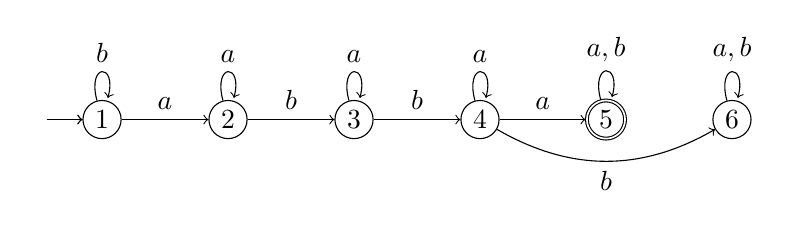
\begin{tikzpicture}[node distance=16mm, every state/.style={minimum size=4mm, inner sep=2pt}]
		\node[state,initial,initial,initial text={}] (1) {$1$};
		\node[state] (2)  [right of=1]  {$2$};
		\node[state] (3) [right of=2] {$3$};
		\node[state] (4)  [right of=3]  {$4$};
		\node[state,accepting] (5)  [right of=4]  {$5$};
		\node[state] (6) [right of=5]{$6$};
		
		\path[->] 
		(1) edge [loop above] node {$b$} ()
		(1) edge node [above] {$a$} (2)
		(2) edge [loop above] node {$a$} ()
	    (2) edge node [above] {$b$} (3)
	    (3) edge [loop above] node {$a$} ()
		(3) edge node [above] {$b$} (4)
		(4) edge [loop above] node {$a$} ()
		(4) edge node [above] {$a$} (5)
		(4) edge [bend right] node [below]{$b$} (6)
		(5) edge [loop above] node [above] {$a,b$} ()
		(6) edge [loop above] node [above] {$a,b$} ();
	\end{tikzpicture}
\caption{automaton6}
\label{fig:error_6}
\end{figure}


\end{document}
